\chapter{The LHCb experiment}
\label{cap:LHCb}

\section{The Large Hadron Collider}

\begin{figure}[t]
	\centering
	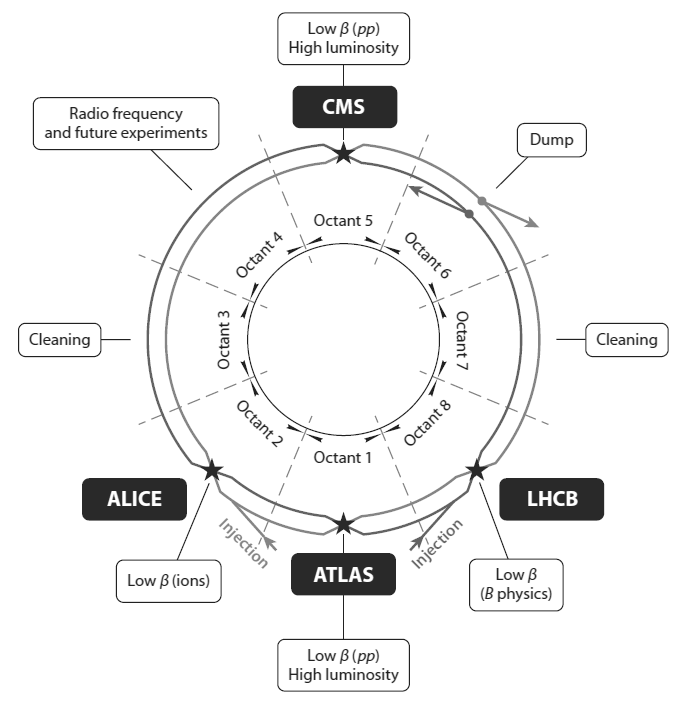
\includegraphics[width=.6\textwidth]{graphics/02-lhcb/lhc_diagram.png}
	\caption[LHC schematic layout.]{Layout of the Large Hadron Collider with its four main experiments \cite{doi:10.1146/annurev-nucl-102010-130438}.}
	\label{fig:2:lhc_diagram}
\end{figure}

At the moment of writing, the Large Hadron Collider (LHC for short) is the largest and most powerful particle collider in the world.
When the LHC was first approved by the European Organization for Nuclear Research (CERN) in 1994, it was originally going to be built with an initial center-of-mass collision energy of \SI{10}{\tev}, with the plan to upgrade it to \SI{14}{\tev} at a later stage;
however, after negotiations with nonmember states, in 1996 the CERN council approved the construction at \SI{14}{\tev} energy in one stage \cite{doi:10.1146/annurev-nucl-102010-130438}.
First collisions were obtained in 2010 at center-of-mass energy of \SI{7}{\tev}, with the current world record of \SI{13}{\tev} being achieved in 2015 after the first Long Shutdown.

LHC is located at the CERN laboratory near Geneva, Switzerland, housed in the underground tunnel previously occupied by the LEP experiment.
Its structure, sketched in Figure \ref{fig:2:lhc_diagram}, consists of two counterrotating rings hosting beams for particle-particle collisions (mainly protons, but LHC is also used for ion collisions).

Four main experiments are stationed at the LHC rings intersection points:
ATLAS and CMS are high-luminosity experiments focused on general purpose proton-proton collisions; ALICE is optimized for lead-on-lead collisions with lower center-of-mass energy and luminosity compared to the former two; finally, LHCb is dedicated on the study of $b$ hadrons and will be the focus of the rest of this Chapter.


\section{The LHCb experiment and detector}

\begin{figure}[t]
	\centering
	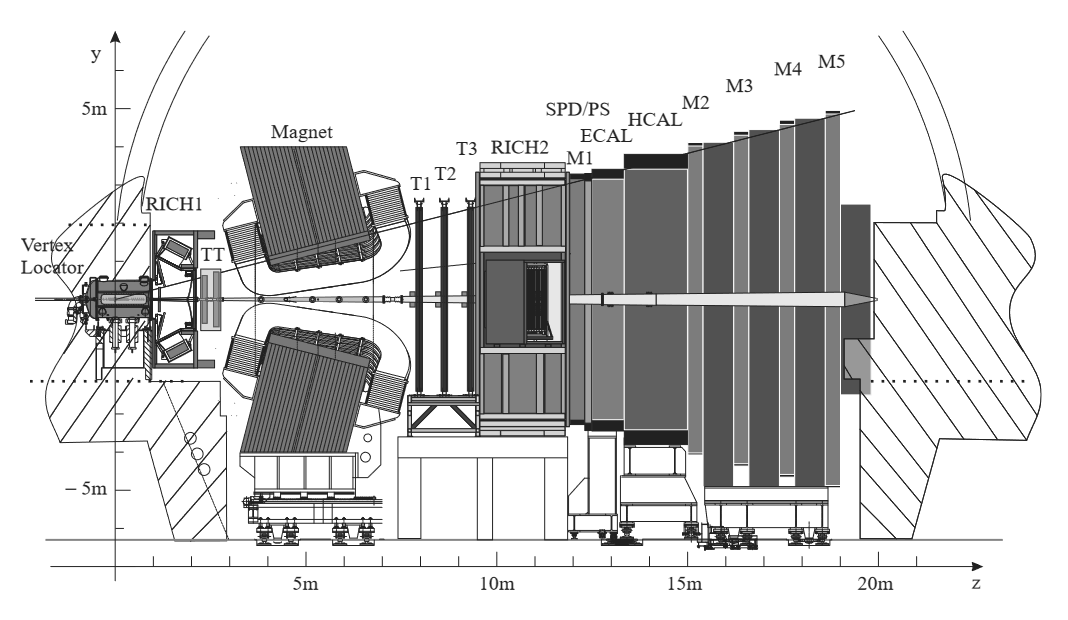
\includegraphics[width=\textwidth]{graphics/02-lhcb/lhcb_diagram.png}
	\caption[LHCb detector side view.]{Side view of the LHCb detector used for LHC Runs 1 and 2 \cite{Antunes-Nobrega:630827}.}
	\label{fig:2:lhcb_diagram}
\end{figure}

LHCb (the \textit{b} stands for \textit{beauty}\footnote{Before settling on the names \textit{top} and \textit{bottom} for the third generation of quarks, the names \textit{truth} and \textit{beauty} were among those proposed. While they never gained enough momentum in the scientific community, echoes of the failed nomenclature are still present in heavy quark vocabulary, for instance in the alternative name \textit{truth} for the \textit{topness} flavour number mentioned in Section \ref{sec:flavour-physics}, as well as in the official name for the LHCb experiment.}) is a single-arm detector designed to study heavy-flavour physics at the LHC, with the main objective of providing precision measurements of CP violation and rare decays of $b$ and $c$ hadrons \cite{Alves:1129809}.

Unlike the other three main experiments at LHC, LHCb has a forward-optimized geometry shown in Figure \ref{fig:2:lhcb_diagram}, with an angular acceptance of $10\div300$ \si{\mrad} in the bending plane and $10\div250$ \si{\mrad} in the non-bending plane.
Such a layout, more reminiscent of fixed target experiments than beam colliders, is motivated by the fact that $b\bar{b}$ pairs produced at high energies are usually collimated in the same forward/backward cone.
A more in-depth look at the tracking and particle identification systems will be taken in Sections \ref{sec:2:tracking} and \ref{sec:2:pid} respectively.
\label{info:LHCb_system}
The standard LHCb coordinate system, used as reference for the rest of this thesis, is a right-handed system centered on the beam interaction point, with the $z$ axis along the the beam pipe and $y$ axis directed vertically upwards.

Elenca i successi.

\subsection{Tracking}
\label{sec:2:tracking}
In order to measure the momenta of charged particles through their bending curve, LHCb employs a dipole magnet consisting of two trapezoidal coils bent at $45^\circ$ on the two transverse sides, seen in Figure \ref{fig:2:lhcb_diagram} around $z\approx \SI{5}{\meter}$ (the magnet is placed so that the line connecting the centers of the pole faces crosses $z=\SI{5.3}{\meter}$).

\begin{figure}[t]
	\centering
	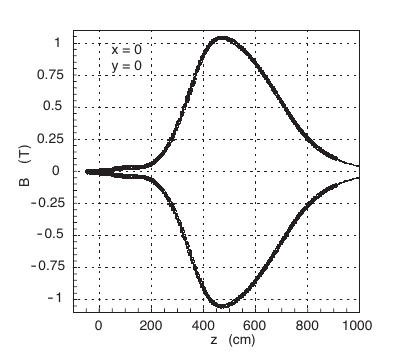
\includegraphics[width=.6\textwidth]{graphics/02-lhcb/b_field_map_z.png}
	\caption{A. \cite{Amato:424338}}
	\label{fig:2:b_field_map_z}
\end{figure}

This magnet provides an integrated field of $\int B dl \approx \pm \SI{4}{\tesla\meter}$ for \SI{10}{\meter} tracks\footnote{The $\pm$ sign is due to the fact that the magnet operates alternatively in up and down polarities, inverting the sign of the magnetic field.} \cite{Amato:424338}.
Most of this field is contained in the $z\in[2.5,7.95]$ \si{\meter} region, with 
a small fraction ($\int B dl \approx \SI{0.12}{\tesla\meter}$) upstream of $z=\SI{2.5}{\meter}$. The field map along $z$, measured with a precision of $4 \times {10}^{-4}$, is shown in Figure \ref{fig:2:b_field_map_z} for $x=y=0$.
Dishomogeneities in the $xy$ plane for fixed $z$ are estimated at $\pm 1\%$ within the LHCb detector acceptance \cite{Alves:1129809}. 

\subsubsection{VELO}

\subsubsection{Tracker Turicensis}
The Tracker Turicensis (TT), also known as Trigger Tracker,

\subsubsection{T stations}

\subsubsection{Track classification}

\begin{figure}[t]
	\centering
	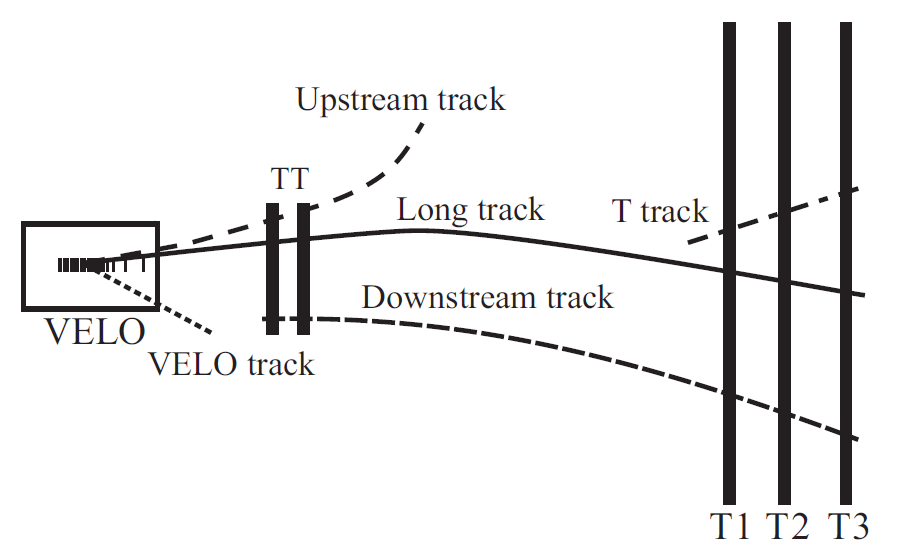
\includegraphics[width=.8\textwidth]{graphics/02-lhcb/Track_Definitions.png}
	\caption{A.}
	\label{fig:2:track_classification}
\end{figure}

Qui tutta la storia delle T track

\subsection{Particle identification}
\label{sec:2:pid}

\subsubsection{RICH}

\subsubsection{Calorimeter}

\subsubsection{Muon system}

\section{The LHCb data flow}
Qui trigger, track reconstruction e tutto il resto.

\section{LHCb detector upgrade for Run 3}

\begin{figure}[t]
	\centering
	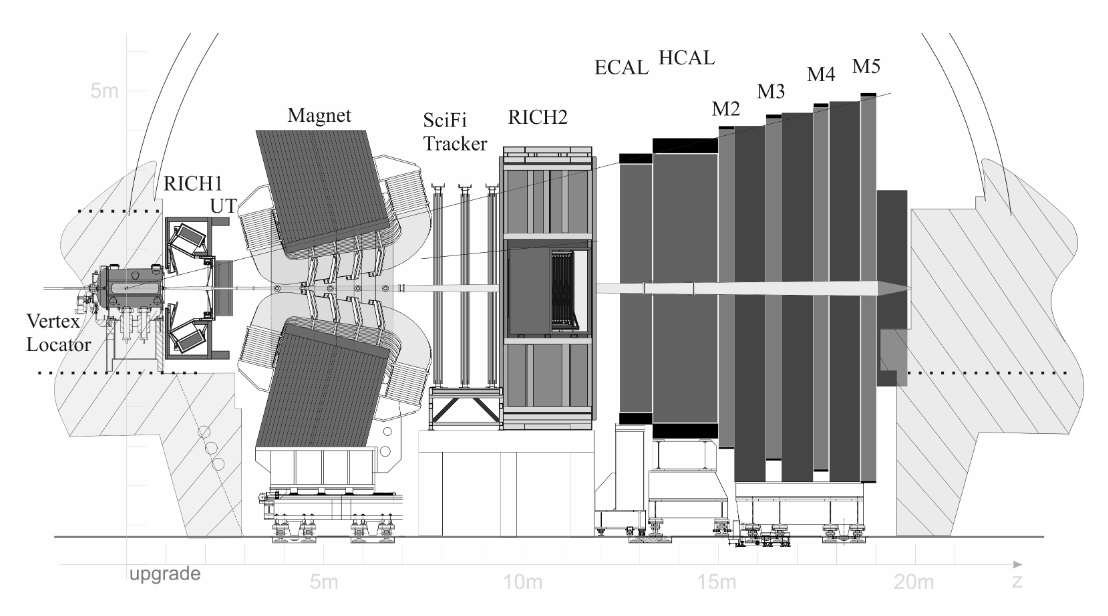
\includegraphics[width=\textwidth]{graphics/02-lhcb/lhcb_diagram_run3.png}
	\caption[LHCb detector side view.]{Side view of the upgraded LHCb detector for future usage in LHC Run 3 \cite{Piucci_2017}.}
	\label{fig:2:lhcb_diagram_run3}
\end{figure}

\section{Data}
Non so se vada qui ma da qualche parte deve andare.